\subsection{OpenMP of the Jacobi Method}
The Jacobi method updates a new matrix from the values of an old one, and it is thus easily parallelizable. The program is paralellized using orphaning in openMP. The \texttt{\#pragma omp parallel} is inside the while loop described above. That has the obvious disadvantage that the worker team will be created and destroyed with each iteration, creating a lot of overhead that will reduce performance. To measure and analyze the performance and scaling behavior of the paralized implementations, we map the speedup as a function of the number of processors/threads used. To investigate the speedup, the program is sent through the Sun Studio Performance Analyzer tool in sequential mode to see the fraction of time f spent in the parallelized region, to facilitate a comparison with Amdahl's law. All experiments in this subsection are run with $N = 10000$, $d = 0.01$ and $k_{max} = 10000$. In all cases and with 1 core, the wall time is $\sim 16$ s, verifying that our parallelization does not have any immediate negative effects on our program.

\begin{equation}
S(P)=\dfrac{T(1)}{T(P)}=\dfrac{1}{(f/P+1-f)}
\end{equation}

S(P) is the speed up. T(1) is the sequential execution time, P is the number of processors, T(P) is the execution time on P processors and f is the parallized fraction of the code. The first implementation only parallelizes the Jacobi update loop. So we have a parallel region before the call to jacobi function and a pragma for in the function itself.

\begin{lstlisting}[caption = While loop of our initial omp program]
while(checksum > d && k < kmax){
			#pragma omp parallel default(none) shared(u,uo,f,N,delta2) private(i,j)
			{
				jacobi_seq(u,uo,f,N,delta2);
			} // end parallel
			checksum = fnorm_squared(u,uo,N);
			for(i = 0; i<N; i++){
				for(j = 0; j<N; j++){
					uo[i][j] = u[i][j];
				}
			} 
			
			k++;
		} 
\end{lstlisting}

The speedup of the initial simple implementation is seen in figure \ref{fig:omp_scale1}. It is seen, that we experience some speed up on more processors, but it does stabilize quickly around 5 threads with a speed up factor of 1.15. The f value of 0.22 is found with the analyzer tool, and it is rather low and clearly much of computation time is not spent in parallel, and when we compare it to Amdahl's law, it is clearly not performing well, most likely due to parallel overhead.


\begin{figure}[h!]
\centering
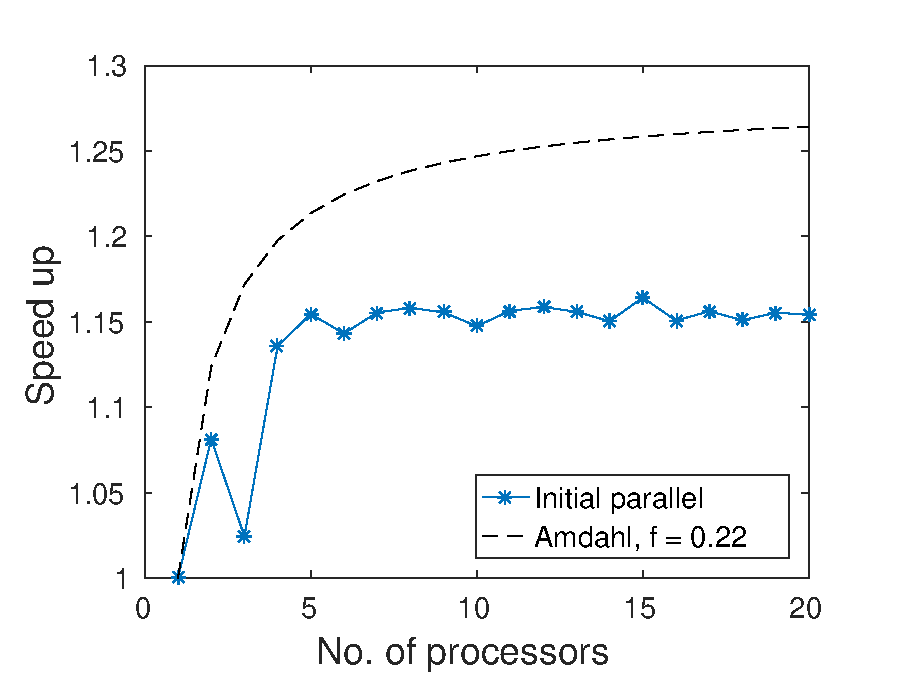
\includegraphics[width = 0.8\textwidth]{fig/speedup_omp.eps}
\caption{Scaling of the first parallelized version.}
\label{fig:omp_scale1}
\end{figure}

We now seek to improve the performance of our OpenMP program. First we realize, that the initial version is only running the Jacobi calculation in parallel, and that the program spent a lot of time on calculating the Frobenius norm and updating the old matrix, about 70 \%. Furthermore, initializing the parallel region in each iteration is not optimal, so we seek to move the parallel region declaration outside the while loop. We created an additional parallel implementation called \texttt{omp2} that deals with these shortcomings. Our while loop for omp2 is as follows.

\begin{lstlisting}[caption = While loop of our optimized (omp2) program]
#pragma omp parallel default(none) shared	(u,uo,f,N,delta2, checksum, k, d, kmax) private(i,j)
				{
				while(checksum > d && k < kmax){
						jacobi_seq(u,uo,f,N,delta2);
						#pragma omp for	private(i,j)  reduction(+:checksum)
						for(i = 1; i <N-1; i++){
							for(j = 1; j<N-1; j++){
								checksum += (u[i][j]-uo[i][j])*(u[i][j]-uo[i][j]);
							}
						}
						#pragma omp for	private(i,j) 
						for(i = 0; i<N; i++){
							for(j = 0; j<N; j++){
								uo[i][j] = u[i][j];
							}
						} 
						#pragma omp master
						{
						k++;
						checksum=checksum/(N*N);		
						}
						#pragma omp barrier
				} // end while 
				
			} // end parallel

\end{lstlisting}


The specific changes are described in the following: The parallel initialization is moved outside the while loop with the shared variables u,uo,f,N,delta2, checksum, k, d and kmax. The Jacobi calculation is parallel using pragma omp for as in the simple version, the checksum is also parallel by using a omp for loop with reduction on checksum, so we do not experience any simultaneous update errors. The update to iteration count k and checksum normalization is inside a pragma omp master directive such that they are only updated once each iteration to ensure the same behavior as the sequential version. In the end we set a barrier to make sure, that the while loop is finished and the loop variables checksum and k updated before starting a new iteration.


We now end up with a much higher parallel fraction f of 0.93, again from the analyzer tool. In figure \ref{fig:omp2_scale} the scaling behavior is seen for the more optimized version. The speed up is clearly much bigger stabilizing at 7 threads with a bit less than a factor 4. It does however not keep up with Amdahl's law, again due to parallel overhead, and the fact that memory initialization is done by the master thread, and used by all threads, which can reduce speedup when the number of cores exceed the number of cores per socket, which in this case is 10.

\begin{figure}[h!]
\centering
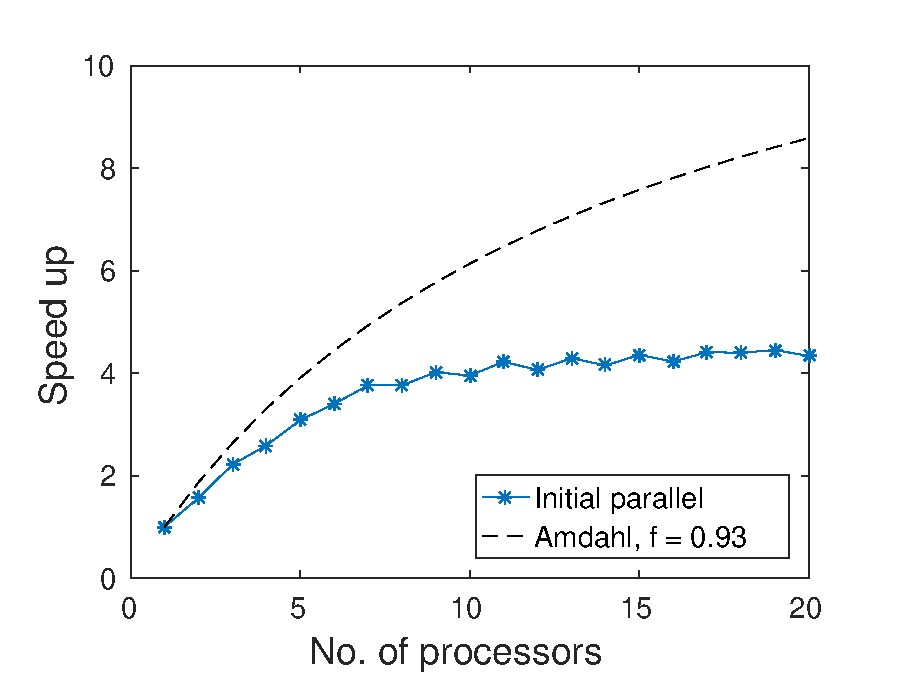
\includegraphics[width = 0.8\textwidth]{fig/speedup_omp2.eps}
\caption{Scaling of the second parallelized version of the whole computational while loop.}
\label{fig:omp2_scale}
\end{figure}

As a final step, we seek to optimize the program even more by implementing a parallelization of the memory allocation and initialization of the matrices to avoid remote memory access when using larger number of threads. This is only relevant when the number of processors exceeds 10 because then processors 10 and above will access data from the other socket. 
We added an if-clause that checks the number of threads and if it is above 10, runs the memory allocation in parallel. We also moved the initialization of the matrices to a parallel region and added pragma fors for the initialization loops.

The way we allocated memory to matrices initially is as follows: 


\begin{lstlisting}[caption = Initial memory allocation]
double ** dmalloc_2d(int m, int n) {
	if (m <= 0 || n <= 0) return NULL;
	double **A = (double **)malloc(m * sizeof(double *));
	if (A == NULL) return NULL;
	A[0] = (double *)malloc(m*n*sizeof(double));
	if (A[0] == NULL) {
		free(A); 
		return NULL; 
	}
	int i;
	for (i = 1; i < m; i++)
		A[i] = A[0] + i * n;
	return A;
}
\end{lstlisting}

With this approach the entire m*n array of matrix values is contiguous meaning everything is stored in a single location.

Since we want different threads to be able to store relevant rows of the matrices to memory locations close to them we need to make sure the calls to malloc are within a parallel region and workshared.
The simplest way to do this is with a pragma omp for as follows:

\begin{lstlisting}[caption = Parallelized memory allocation]

double ** dmalloc_2d_opt(int m, int n) {
	if (m <= 0 || n <= 0) return NULL;
	double **A = (double **)malloc(m * sizeof(double *));
	if (A == NULL) return NULL;
	//A[0] = (double *)malloc(m*n*sizeof(double));	
	#pragma omp parallel default(none) shared (A, m, n)
	{
		int i;
		#pragma omp for	private(i) 
		for (i = 0; i < m; i++)
			A[i] = (double *)malloc(n*sizeof(double));
	}
	return A;
}
\end{lstlisting}


We call this version \texttt{omp3}. The speedup plot can be seen in figure \ref{fig:omp3_scale}. It should be noted that for this plot we fit a line for our speedup curve and computed the f value from the fitted line. Although there is a small dropoff at 19 and 20 threads, the observed f of 0.955 effectively represents the proportion of the problem that we managed to 'perfectly' parallelize.  

As seen from figure \ref{fig:omp3_scale} the increase in speedup continues above 10 processors, which was not the case with \texttt{omp2}.

\begin{figure}[h!]
\centering
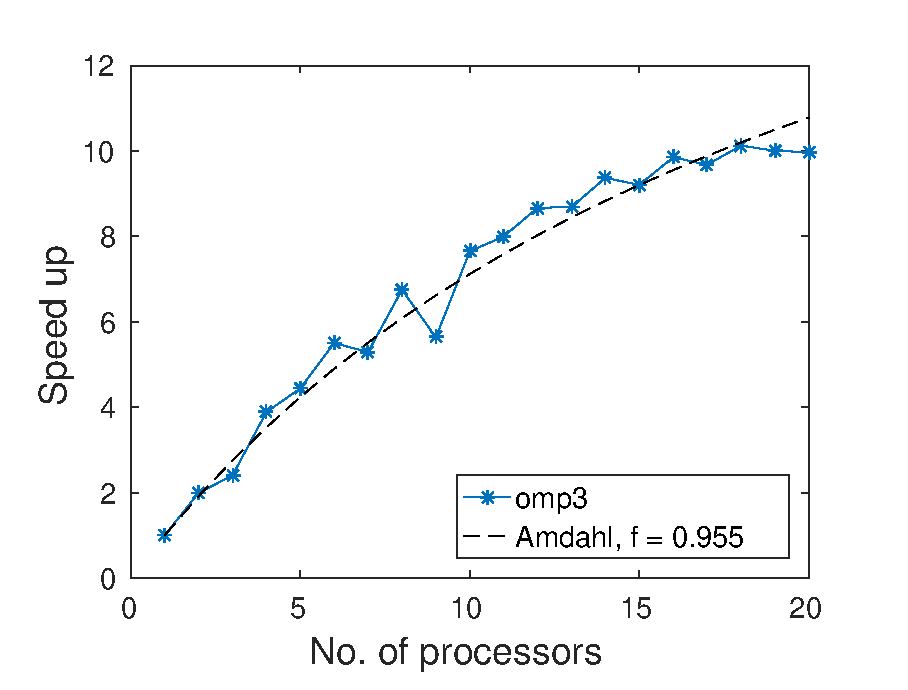
\includegraphics[width = 0.8\textwidth]{fig/speedup_omp3.eps}
\caption{Speed-up scaling of the third parallelized version, which includes parallel memory allocation.}
\label{fig:omp3_scale}
\end{figure}


Lastly, we compare the efficiency of our three different parallel implementations. This is done by computing the efficiency, which is the speed up increase per added thread. Figure \ref{fig:omp_eff} clearly shows how different the efficiency curves are for the three different implementations. The simple implemenation clearly falls of right at the beginning, where the efficiency drops to a little higher than 50\% already at thread nr. 2, which is obvious since the speed up factor is only slightly above 1. For the case of the more optimized implementation, it is clear that the omp3 version reigns supreme, and it does not reach 50\% effiency before the 19th to 20th added thread, which makes sense, since we saw in the speed-up scaling that it started to stagnate at that point. Meanwhile the omp2 parallelization already reaches 50\% around 7-8 threads.

\begin{figure}[h!]
\centering
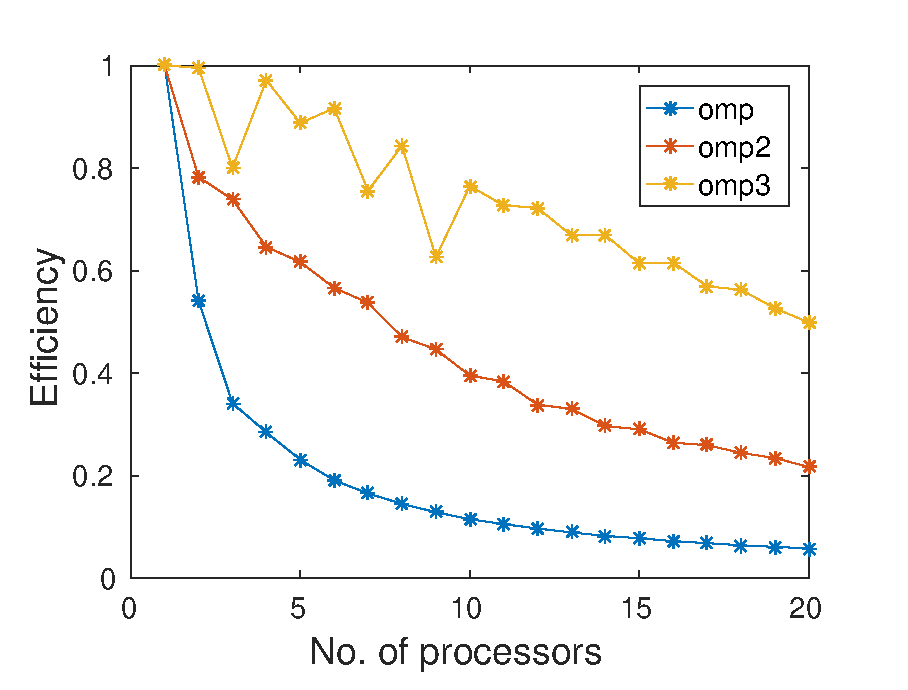
\includegraphics[width = 0.8\textwidth]{fig/efficiency_omp_omp2_omp3.eps}
\caption{Effiency plot of the three parallel versions.}
\label{fig:omp_eff}
\end{figure}
